
%(BEGIN_QUESTION)
% Copyright 2006, Tony R. Kuphaldt, released under the Creative Commons Attribution License (v 1.0)
% This means you may do almost anything with this work of mine, so long as you give me proper credit

One of the most fundamental relationships in the study of electricity is {\it Ohm's Law}.  This mathematical expression relates the flow of electric charge ($I$, which we call {\it current}) to electromotive potential ($V$, which we call {\it voltage}) and opposition to charge flow ($R$, which we call {\it resistance}):

$$\includegraphics[width=15.5cm]{i00086x01.eps} I = {V \over R} \hbox{\hskip 10pt} \hbox{(For all conditions)}$$

The relationship between {\bf liquid} flow rate, pressure drop, and ``resistance'' for a piping restriction (orifice, throttling valve, pipe bend, etc.) is not as simple.  No single mathematical expression is sufficient to predict flow rates for all conditions:

$$\includegraphics[width=15.5cm]{i00086x02.eps}$$

$$Q = {{P_1 - P_2} \over R_1} = {\Delta P \over R_1} \hbox{\hskip 10pt}  \hbox{(For laminar flow conditions only)}$$

\vskip 10pt

$$Q = \sqrt{{P_1 - P_2} \over R_2} = \sqrt{\Delta P \over R_2} \hbox{\hskip 10pt}  \hbox{(For turbulent flow conditions only)}$$

Shunt resistors may be used as electric current-measuring elements, producing a voltage drop in precise proportion to the current through it.  All we need to know is the shunt resistance, and we may infer current by measuring voltage.  In a similar manner, orifices may be used as liquid flow-measuring elements, producing a pressure drop that varies with the amount of flow passing through it:

$$\includegraphics[width=15.5cm]{i00086x03.eps}$$

Given the ``Ohm's Law'' equations shown for liquid flow, identify what we would have to know before using an orifice as an accurate liquid flow-measuring device, and how we would be able to obtain that information.  Also identify the type of sensing instrument we would need to measure the pressure, so we could infer flow rate from its reading.

\underbar{file i00086}
%(END_QUESTION)





%(BEGIN_ANSWER)

Here, what we do not know about the flow-measurement scenario is the flow regime (laminar or turbulent), and also what the ``resistance'' of the fluid restriction is.  Of course, the Reynolds number for our flowstream will indicate its regime status, and the $R$ factor for the orifice may be either determined experimentally or derived from orifice equations (available in any exhaustive reference book).

\vskip 10pt

The proper pressure-sensing instrument to use for fluid flow is a {\it differential pressure} instrument, such as a DP cell or DP gauge, or perhaps even a mercury manometer.


%(END_ANSWER)





%(BEGIN_NOTES)

In case anyone asks, I use subscripts to distinguish the ``resistance'' values $R_1$, $R_2$, etc. in order to show that the ``resistance'' factor will be different for each flow regime.

%INDEX% Physics, dynamic fluids: Resistance of liquid flow component

%(END_NOTES)


